\chapter{Experimental part: Exploratory data analysis / TODO}
\label{chap:dataexplore}
In this chapter we will explore the data we have, create several new features from existing ones, visualize and discover the relationships between them. Most of the figures and tables for this chapter you can find in \nameref{appendix}.\\

Here we often refer to a \textit{meta name} field in the dataset. It may takes five values: \textit{name}, \textit{startDate}, \textit{location}, \textit{description} and \textit{noEvent}. Also we use the term \textit{event component} which is applied to all meta names excluding \textit{noEvent}.


\section{Feature engineering}
Before we start exploring the data we would like to extract several new features. We will work on the following types of features: 

\begin{itemize}
\item \textit{Textual features} related to an original text of the event components.
\item \textit{Spatial features} related to X and Y coordinates of the web element on the page. X and Y are coordinates of a visual block on the real rendered page. 
\end{itemize}

In section \nameref{sec:css} we already extracted several \textit{Visual features} from the CSS properties. We divided into 3 parts a value of color, the font family and properties measured the pixels. 

\subsection{Textual features}

An original textual feature is a text contained in a web element. For the event name, location and start date, it's a quite short string. For a description is much longer text. That's why the first extracted feature is a \textit{length of the text}. On the picture \nameref{fig:distrTextByMeta} you distribution of the text length differs among meta names. \\

After we extracted the text length, we noticed that the date and location meta names usually contain more digits than name and description. So we extracted also the number of digits in a text. See \nameref{fig:distrDigitsByMeta}.\\

By analogy, we extracted also number of uppercase letter, white spaces, digit proportion and a number of punctuation marks. See the rest of the figures in \nameref{appendix}.



\begin{figure}[h]
\begin{subfigure}{1\textwidth}
  \centering
  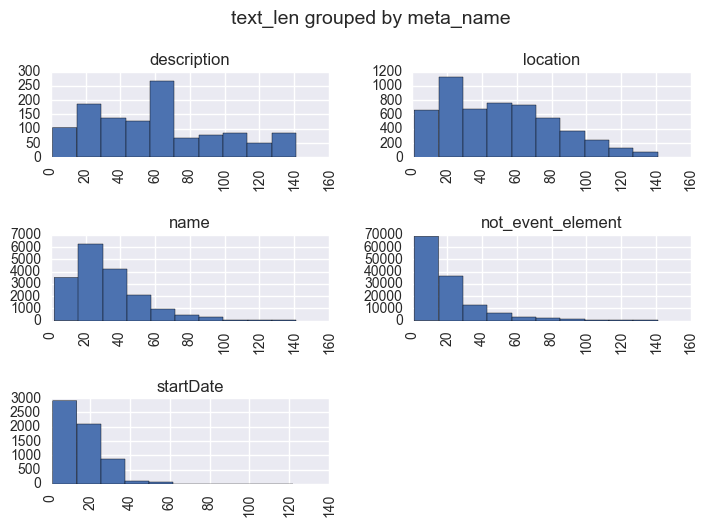
\includegraphics[width=1.0\textwidth]{figures07/distrTextByMeta}
  \caption{Histogram}
\end{subfigure} \\
\begin{subfigure}{1\textwidth}
  \centering
  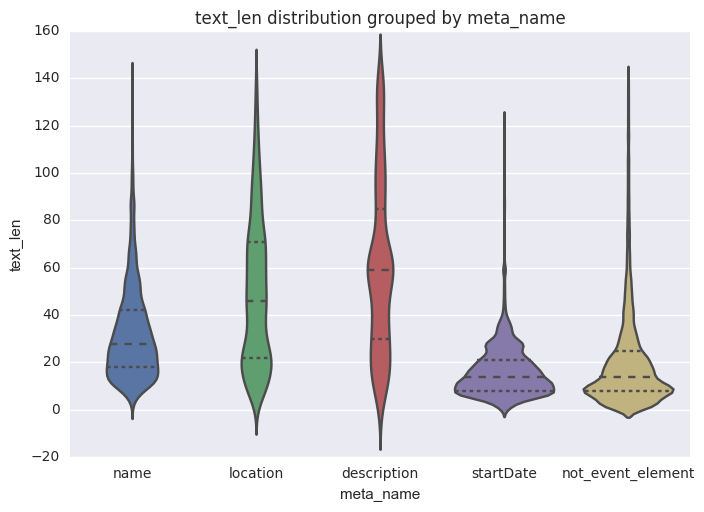
\includegraphics[width=1.0\textwidth]{figures07/distrTextByMeta_violin}
  \caption{Violin plot}
\end{subfigure}
\caption{Distribution of text length by meta name}
\label{fig:distrTextByMeta}
\end{figure}


\begin{figure}[h]
\begin{subfigure}{1\textwidth}
  \centering
  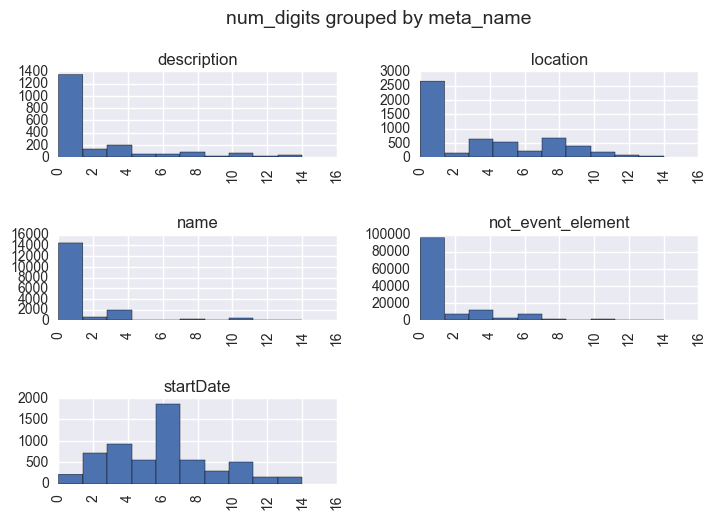
\includegraphics[width=1.0\textwidth]{figures07/distrDigitsByMeta}
  \caption{Histogram}
\end{subfigure} \\
\begin{subfigure}{1\textwidth}
  \centering
  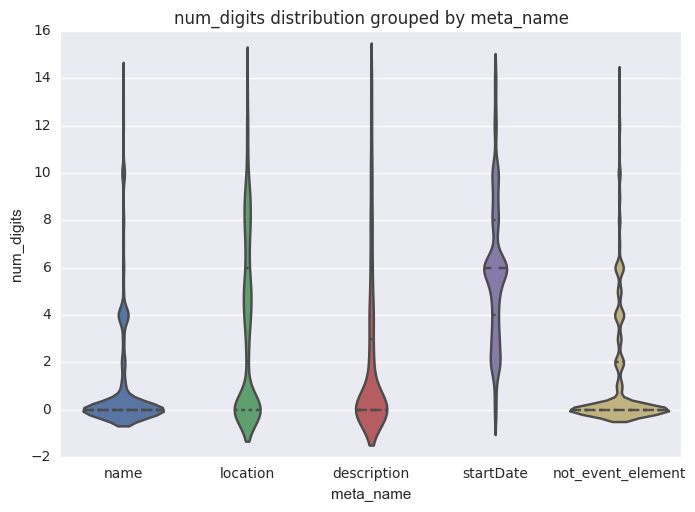
\includegraphics[width=1.0\textwidth]{figures07/distrDigitsByMeta_violin}
  \caption{Violin plot}
\end{subfigure}
\caption{Distribution of digits number by meta name}
\label{fig:distrDigitsByMeta}
\end{figure}

Therefore we created six additional features from one textual field: text length, number of punctuation marks, number of digits, digits share, number of upper case letters, number of white spaces. You can see that visually they distinguish meta names well. The difference in basic statistics you can find in table \nameref{table:textualDistr}. \\

When we build different classification models in the next chapter, we will also calculate a \textit{tf-idf weighting matrix} in ofrder to reflect the importance of every word in a text.

\subsection{Spatial features}

Here we will work on two original coordinates X and Y of a visual blocks. The visual block is a rectangle on a webpage where the web element is located. Also, we will use two other related features: block width and block height. The precise meaning of X,Y features as follows: X pixels means horizontal position on page from left side, and Y pixels means vertical position on page from top side. That means that X and Y are coordinates of the left upper corner of the corresponding visual block. For example, see \nameref{fig:startDateXY}.\\

The first feature we created, is an ultimate X and Y which are centers of the visual block rather then left upper corner. Our guess was that these two features better represent the location on the page.\\

Then we applied K-means clustering algorithm with to assign the cluster label for every row. The idea here was to attempt the visual block on a page where every component might appear. We learned the model for sub datasets for every meta name. Unfortunately this experiment wasn't successful, because it appears that centered X and Y don't have a clustering structure. Rather the elements can appear almost anywhere on a page with only small deviation in means. See figure \nameref{fig:nameXYCluster8}. There are some difference in basic statistics of X and Y for different meta names, but the standard deviation is so high that it can't be considered as a significant result. See the table \nameref{table:spatialDistr}. \\

We can make several conclusions on the spatial features:
\begin{itemize}
    \item Visually it separates the mate names badly.
    \item The average of X coordinate differs for all meta names, but the standard deviation is very high.
    \item Both, the visualization and summary statistics say the following things: the name is located higher, the start date is more on the left side, the start date is usually more lefter than the location, and description is usually below. This is quite expected.   
\end{itemize}

\begin{figure}[h]
\begin{center}
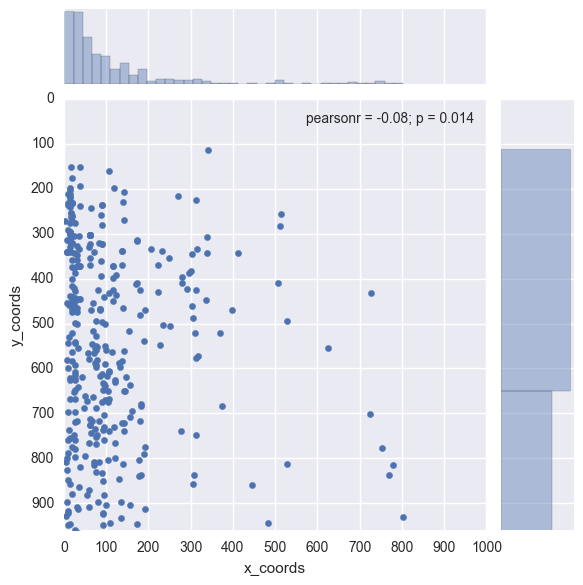
\includegraphics[width=.6\textwidth]{figures07/startDateXY}
\caption{The distribution of original X and Y for an event start date}
\label{fig:startDateXY}
\end{center}
\end{figure}


\begin{figure}[h]
\begin{center}
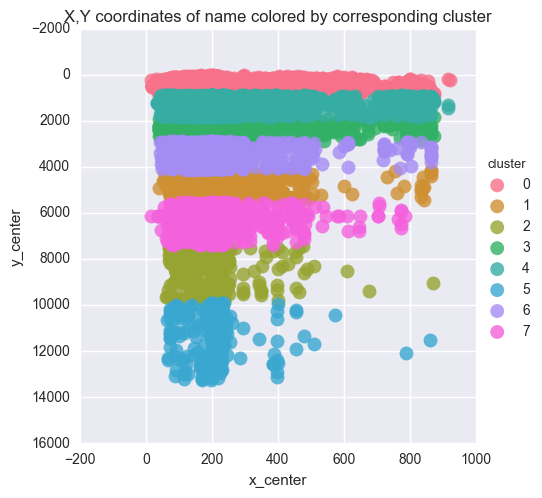
\includegraphics[width=.6\textwidth]{figures07/nameXYCluster8}
\caption{Unsuccessful clustering of X,Y center of the blocks for event name, K = 8}
\label{fig:nameXYCluster8}
\end{center}
\end{figure}    

\section{Final dataset}
The final dataset after the cleaning and feature engineering is a table of 168K rows and 32 columns. Let's look at its main properties: 

\begin{itemize}
    \item The list of columns in the dataset: \nameref{table:featurelist}.
    \item It's cleaned of outliers, frequent domains, multi-events pages and inconsistency. 
    \item It contains 33K unique URLs, and  4000 domain names. 
    \item There are in average 45 URLs per one domain name. 
    \item We have 137K rows related to a random elements on the webpage, 18K for a event's name, 6K for a start date, 6K for location, and 2K for description. In sum, 32K rows containing features of event components. 
    \item There a in average 1.8 event components out of 4 on a webpage. 
    \item There are the most popular combinations of event components fro one URL. 
    \begin{itemize}
        \item \textit{name} 8335
        \item \textit{location, name} 2863 
        \item \textit{name, startDate} 2522 
        \item \textit{location, name, startDate} 1735
    \end{itemize}
    Top 10 list of combinations you may find in table \nameref{table:top10comb}.
    \item We have 30 numeric features and 4 textual. Additionaly, we will include \textit{idf-idf} matrix later.
    \item We replaced outliers of numerical features with the NaN. We fill the missing values with the corresponding average values.  
    \item 
\end{itemize}


\begin{table}[h]
\begin{center}
{\renewcommand{\arraystretch}{1.2}
\begin{tabular}{| p{6cm} | p{6cm} |}
\hline
\textbf{DOM}   &   \textbf{CSS}\\
\hline
URL of the page    &    Color (three chanells)\\
Meta name (name, startDate, description, location, no\_event)    &    Text alignment (center, left, right, etc)    \\
Text of the web element    &    Property of the block view    \\
HTML tag    &    The level font weight    \\
Number of siblings in a DOM tree    &    Padding    \\
Number of childs in a DOM tree    &    Font family (Verdana, Arial, etc)    \\
    &    Font size \\
    &    The language of the page \\
    
    &    \textit{+ 270 other CSS features} \\
\hline
\textbf{Visual}   &   \textbf{Textual}  \\
\hline
X and Y coordinate on the rendered picture    &    Length of the text inside the block    \\
X and Y coordinate of the center of a visual block    &    Number of punctuation marks in text    \\
Visual block height     &    Number of digits in text    \\
Visual block width        &    Number of digits/text length    \\
Height in a browser     &    Number of upper case letters    \\
Width in a browser     &    Number of whitespaces    \\

     &    \textit{+ tf-idf matrix}    \\
\hline
\end{tabular}}
\caption{List of features}
\label{table:featurelist}
\end{center}
\end{table}    



\begin{table}
\begin{center}
{\renewcommand{\arraystretch}{1.5}
\begin{tabular}{| p{8cm} | p{2cm}|}
\hline
\textbf{Combination}	&	\textbf{Count}\\
\hline
['name']	&	8335\\
\hline
['location', 'name']	&	2863\\
\hline
['name', 'startDate']	&	2522\\
\hline
['location', 'name', 'startDate']	&	1735\\
\hline
['description', 'name']	&	730\\
\hline
['description', 'name', 'startDate']	&	548\\
\hline
['description', 'location', 'name']	&	485\\
\hline
['description', 'location', 'name', 'startDate']	&	293\\
\hline
['name', 'startDate', 'startDate']	&	246\\
\hline
['location', 'name', 'startDate', 'startDate']	&	125\\
\hline
\end{tabular}}
\caption{Top 10 combinations of event component for one URL}
\label{table:top10comb}
\end{center}
\end{table}	

\section{Analysis of features}
Let's look at other fields of the dataset and visualize with the grouping by the meta name.    

\begin{table}
\begin{center}
{\renewcommand{\arraystretch}{1.5}
\begin{tabular}{| p{0.8cm} | p{2cm}|  p{2cm}|  p{2.3cm}|  p{2.3cm}|  p{2.4cm}|}
\hline
\textbf{stat}	&	\textbf{color\_r}	&	\textbf{font\_size}	&	\textbf{font\_weight}	&	\textbf{digits\_share}	&	\textbf{block\_height}\\
\hline
count	&	167872.0	&	167872.0	&	167872.0	&	167872.0	&	167872.0\\
\hline
mean	&	76.396201	&	14.69536	&	455.510746	&	0.112503	&	26.359833\\
\hline
std	&	84.989934	&	4.15742	&	129.067880	&	0.225118	&	18.612600\\
\hline
min	&	0.0	&	0.0	&	100.0	&	0.0	&	0.0\\
\hline
25\%	&	4.0	&	13.0	&	400.0	&	0.0	&	16.0\\
\hline
50\%	&	51.0	&	14.0	&	400.0	&	0.0	&	19.0\\
\hline
75\%	&	125.0	&	16.0	&	400.0	&	0.117021	&	31.0\\
\hline
max	&	255.0	&	100.0	&	900.0	&	1.0	&	194.0\\
\hline
\end{tabular}}
\caption{Summary statistics for some numerical features}
\label{table:sumstatnum}
\end{center}
\end{table}	
















\section{Visualization}



